%        File: agree.tex
%     Created: Fri Mar 24 09:00 AM 2017 E
% Last Change: Fri Mar 24 09:00 AM 2017 E
%
% arara: pdflatex: {options: "-draftmode"}
% arara: biber
% arara: pdflatex: {options: "-draftmode"}
% arara: pdflatex: {options: "-file-line-error-style"}
\documentclass[MilwayThesis]{subfiles}

\begin{document}
In the preceding chapters, I presented an explanation partially of why resultatives cannot be derived in French(-type) languages.
Without further comment, however, this explanation seems to wrongly predict that depictives and copular clauses are also ruled out in French.
In this chapter, I will modify my proposal so that this prediction is removed.
However, rather than modifying any of the claims and hypotheses I have made thus far, I will clarify another portion of the grammar, namely, the Agree operation.
With this clarification, will be able to rule out resultatives in French without ruling out depictives and copular clauses.
Furthermore, the clarified grammar will provide a straightforward explanation of \textit{wanna}-contraction in English.

\section{The faulty predictions: *depictives, *copular clauses}
In order to account for the lack  of resultatives in French(-type languages), I have argued that DP movemment from a small clause is barred in these languages.
The fact that (\textit{e.g.}) French allows copular clauses and depictives, however, means that this restriction must only hold in would-be resultative derivations.
In other words, our grammar should generate \cref{ex:FreCop} and \cref{ex:FreDep} but not \cref{ex:FreRes}.
\exg. \label{ex:FreCop}Jeanne est grand -e.\\
Jeanne is tall -FSg\\
``Jeanne is tall.''

\exg. \label{ex:FreDep}Marie mange la viande crue\\
Marie eats the.FSg meat raw.Fsg\\
``Marie eats meat raw''

\exg.* \label{ex:FreRes}Sophie a martell\'e le m\'etal plat.\\
Sophie \textsc{aux} hammered the.MSg metal flat.MSg\\
``Sophie hammered the metal flat.''

Consider the case of the copular clause \cref{ex:FreCop}, whose structure is given in \cref{fig:FreCop}
\begin{figure}[h]
	\centering
\begin{forest}
  nice empty nodes,sn edges,baseline,for tree={
    calign=fixed edge angles,
  calign primary angle=-30,calign secondary angle=70}
  [$\delta$
    [DP$_\varphi$[Jeanne,roof]]
    [$\gamma$
      [T$_\varphi$]
      [$\beta$
	[$\langle$DP$_\varphi\rangle$]
	[$\alpha$
	  [adj$_\varphi$]
	  [\textsc{grand}]
	]
      ]
    ]
  ]
\end{forest}
	\caption{Simplified structure of a French copular clause}
	\label{fig:FreCop}
\end{figure}
French \textit{adj} has a single $\varphi$-set, meaning it can only label if it is strengthened by agreement.
In the case of resultatives, DP movement out of a small clause bleeds agreement with \textit{adj}.
If this is true of \cref{fig:FreCop}, then $\alpha$ and $\beta$ would be unlabelable.
Similar remarks apply to depictives as well.

This line of thinking is based on the implicit premiss that lower copies are invisible to Agree as well as Label.
We could save \cref{ex:FreCop}, by hypothesizing that lower copies are visible to Agree and invisible to Label, but this would predict that French generates resultatives, clearly an unwanted result.
The solution to this puzzle is to say that lower copies are invisible to Agree only under certain circumstances.
The next section will hypothesize the nature of these ``certain circumstances'' by clarifying the Agree operation.

\section{The nature of the Agree operation}

In \cref{sec:nonstandard}, I stated my assumption that syntactic agreement occurs outside of the Narrow Syntax.
Unsurprisingly, this assumption requires additional specificity.
If we take Agree to be an operation, we can ask where it fits in the grammatical architecture.
By hypothesis, it operates on the output of the Narrow Syntax, and it must operate before labelling.
Furthermore, its effects are seen in externalization.
These considerations suggest that Agree is part of Transfer, that is, it operates on derived syntactic objects before they are sent to the interfaces.
This is represented in \cref{fig:SepCycles}.
%Crucial to both label theory in general and its application in this thesis, is syntactic agreement.
%The highest XP in a given chain must agree with its sister YP in order to converge, and a subset of functional heads must agree in order to label (\textit{e.g.}, English T$_\varphi$).
%In this chapter I will discuss the theory of agreement, as it relates to labeling and show how the version of agree required for labeling avoids an undergeneration issue apparently predicted for predicative adjectives in French-type languages.
%
%Agreement is required in label theory to account for (\textit{e.g.},) Subject-TP structures as in \Next.
%\ex. [$_\alpha$ DP$_\varphi$ [$_\beta$ T$_\varphi$ ZP]]
%
%The labels of both $\alpha$ and $\beta$ depend on agreement between the subject and T.
%Since $\alpha$ is a Phrase-Phrase structure, its label will be $\langle\varphi,\varphi\rangle$ provided DP and T agree for $\varphi$.
%This agreement also renders $\beta$ labelable, since, prior to agreement, English T$_\varphi$, with an incomplete $\varphi$-set, is too weak to label \parencite{chomsky2013problems}.
%Agreement has the effect of strengthening T such that it can label.
%
%To understand how Agree and Label interact, we must first consider what sort of operations they each are abstracting away from their actual implementations.
%Both take syntactic objects as inputs and operate on them iteratively and locally.
%This means that labeling a structure like \Last requires labeling all of its substructures (Iterativity) and that labeling $\beta$ depends solely on the properties of $\beta$ (Locality).
%The same, then, is true for Agree, which iteratively considers each substructure and performs agreement is the conditions for agreement are met.
%
%Because labeling is sometimes contingent on agreement, the calculation of the latter must precede that of the former.
%Assuming both Agree and Label occur after narrow syntax and before transfer to CI, this leaves us with two possibilities for ordering the two operations.
%Either (i) individual iterations of Agree and Label are ordered with respect to each other forming a single Agree+Label cycle or (ii) Agree and Label each has its own cycle, and those cycles are ordered with respect to each other.
%To decide between these two alternatives we can consider how Agree and Label interact with other components of grammar, specifically the SM and CI interfaces.
%By hypothesis, Label feeds interpretation at CI but not at SM.
%Agree, on the other hand, feeds Label and interpretation at SM.
%This asymmetry points to the second alternative, where narrow syntax feeds an Agree cycle, which feeds SM interpretation and Label as in figure \ref{fig:SepCycles}.
%The first alternative, in which Agree and Label are bundled into a single cycle as shown in figure \ref{fig:OneCycle}, predicts that both Label and Agree feed both interfaces, which is not what we seem to see in the data. 
\begin{figure}[h]
  \centering
  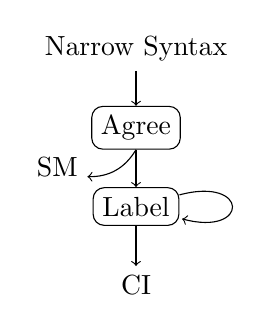
\begin{tikzpicture}
    \node (syn) at (1,3) {Narrow Syntax};
    \node[draw,rounded corners] (agree) at (1,2) {Agree};
    \node[draw,rounded corners] (label) at (1,1) {Label};
    \node (SM) at (0,1.5) {SM};
    \node (CI) at (1,0) {CI};
    \path[->](syn)	edge			(agree)
	   (agree.south)	edge			(label)
			  edge [bend left]	(SM)
	  (label)		edge [loop right]	()
			  edge			(CI);
  \end{tikzpicture}
  \caption{The position of Agree in the grammar}
  \label{fig:SepCycles}
\end{figure}

This much is an almost unavoidable result of my assumtions and the general empirical facts, but we require further hypotheses to arrive at the predictions we need.
The first hypothesis is that Agree feeds some operation that renders lower copies invisible to Label.
This could be a deletion operation, an impoverishment operation, or even a cloaking operation, it's not important, but crucially, it is this operation that renders a lower copy invisible to label.
Presumably the effects of this operation will also be felt at the SM interface.
More on that in \cref{sec:wanna}.

If the Agree operation, in a sense, determines whether a given SO is visible to Label, what determines whether an SO is visible to Agree.
Supposing the input to an Agree-cycle is a a phase P, I hypothesize that all and only those SO's that are \textit{contained} by P are visible to that cycle.
This may seem like a trivial hypothesis, but given the definition of ``SO'' and ``contain'' that I will adopt, it makes actual empirical predictions.

My definition will depend on making the distinction between syntactic objects and their instances.
This type of distinction has been made throughout the development of generative syntax, but perhaps the best known iteration comes in the notion of a chain.
In LGB, for instance, each nominal in an S-Structure was associated with a sequence of grammatical functions that represent its derivational history.
This sequence was called a function chain.
So, in the passive S-structure \cref{ex:passiveSStruct}, \textit{Jennifer} is associated with the chain \cref{ex:PassiveChain}.
\ex.\label{ex:passiveSStruct} Jennifer$_i$ was served $t_i$.

\ex.\label{ex:PassiveChain} $\langle\left[\text{NP,S}\right], \left[\text{NP,VP}\right]\rangle$

There is a sense in which the chain was the real grammatical object in LGB and later systems, as filters like the $\theta$-criterion and the Case filter were satisfied by chains rather than their individual links.
So, \textit{Jennifer} in \cref{ex:passiveSStruct} has a $\theta$-role because a link in its chain ([NP, VP]) has a $\theta$-role
Following \textcite{collins2016formalization}, I replace the chains and links with syntactic objects and occurrences defined below.
\begin{defn}
  X is a \textit{syntactic object} (SO) iff\\
    X is a lexical item, or\\
    X is a set of syntactic objects. \parencite[Modified from][]{collins2016formalization}
  \label{def:so}
\end{defn}
\begin{defn}
  The \textit{position} of \I{SO}n in \I{SO}1 is a path, a sequence of syntactic objects $\langle\text{SO}_1,\text{SO}_2,\dots,\text{SO}_n\rangle$ where for all $0 < i < n$, $\text{SO}_{i + 1} \in \text{SO}_i$. \parencite{collins2016formalization}
  \label{def:position}
\end{defn}
\begin{defn}
  B \textit{occurs} in A at position P iff P = $\langle\text{A},\dots,\text{B}\rangle$. We also say B has an occurrence in A at position P (written \I{B}P).
  \label{def:occurrence}
\end{defn}

Consider the abstract syntactic object and its tree representation below in \cref{ex:AbstractSO} and \cref{fig:AbstractTree}, respectively.
\ex.\label{ex:AbstractSO} $\left\{ \text{X}, \left\{ \text{Y} \left\{ \text{X}, \text{Z} \right\} \right\} \right\}$

\begin{figure}[h]
	\centering
	\begin{forest}
	  nice empty nodes,sn edges,baseline,for tree={
	    calign=fixed edge angles,
	    calign primary angle=-30,calign secondary angle=70
	  }
	  [$\alpha$
	    [X]
	    [$\beta$
	      [Y]
	      [$\gamma$
		[X]
		[Z]
	      ]
	    ]
	  ]
	\end{forest}
	\caption{A Tree representation of \cref{ex:AbstractSO}}
	\label{fig:AbstractTree}
\end{figure}

Based on the definitions above, we can say the following things about \cref{ex:AbstractSO}:
There are six SOs represented in \cref{ex:AbstractSO}: three lexical items (X, Y, Z) and three sets of SOs ($\alpha$, $\beta$, $\gamma$).
There is a single SO, X, with two occurrences in \cref{ex:AbstractSO}:
At $\langle \alpha, \text{X}\rangle$, and at $\langle \alpha, \beta, \gamma, \text{X}\rangle$

With this contrast between SOs and occurrences, we can limit the domain of Agree to complete chains without stipulating the existence of chains.
Consider the structure in \cref{ex:AbstractSO}, assuming that Y is a phase head. 
At a given stage of a derivation, it is reasonable to assume that the computation must track two sets of SOs: The set of SOs in the derivation (\textsc{Terms}$_\text{SO}$), and the set of active SOs (\textsc{Active}$_\text{SO}$).
For \cref{ex:AbstractSO}, the two sets are given in \cref{ex:AbstractTermsActive}.
\ex. \label{ex:AbstractTermsActive}
\a. \textsc{Terms}$_\alpha$ = $\left\{ \text{X}, \text{Y}, \text{Z}, \alpha, \beta, \gamma  \right\}$
\b. \textsc{Active}$_\alpha$ = $\left\{ \text{X}, \text{Y}, \alpha, \beta \right\}$

We can determine the input to Agree, then, by computing the set difference between the two sets as shown in \Next.
\ex.\label{ex:AbstractAgrInput} $\textsc{Terms}_\alpha \setminus \textsc{Active}_\alpha = \left\{ \text{Z}, \left[ \text{X}, \text{Z} \right] \right\}$ 

Note that X, which has moved to [Spec Y] is not a member of the input to Agree, despite the fact that there is a member of the input which has X as a member.
As such, X is invisible to Agree and Label.
With that understood in the abstract, we can consider the concrete cases of copular clauses and resultatives.


\section{Correct predictions: French small clauses saved}\label{sec:FreSaved}

If we take resultatives and depictives to be minimally different, we can begin to investigate the source of the contrast in grammaticality between the two.
Both are secondary predication constructions, consisting of an eventive VP and a stative small clause.
The difference between the two is the semantic relation between the event and state.
Roughly speaking, resultatives describe an event causing a state, while depictives describe an event coinciding with a state.
I have chosen, following \textcite{kratzer2004building} and \textcite{pietroski2005events}, to assume a \textit{res} head that encodes causation, but I see no compelling reason to assume a \textit{dep} head to encode coincidence.
So, a depictive VP has the structure represented in \cref{fig:FreDepVP}.
\begin{figure}[h]
	\centering
	\begin{forest}
		nice empty nodes,sn edges,baseline
		[AgrOP
			[DP [la viande,roof,name=specagro]]
			[
				[AgrO]
				[VP
					[VP
						[mange]
						[DP,name=theme]
					]
					[SC
						[DP,name=scsubj]
						[crue]
					]
				]
			]
		]
		\draw[->] (scsubj) to[out=south, in=south] (theme);
		\draw[->] (theme) to[out=south west, in=south] (specagro);
	\end{forest}
	\caption{A depictive VP}
	\label{fig:FreDepVP}
\end{figure}
As for the coincidence interpretation, I will postpone that discussion until a \cref{sec:coincidence}.
Since resultative structures differ from depictives crucially with respect to the presence of a \textit{res} head, we would expect the contrast in grammaticality to follow from that difference.
To begin, let's compare the two relevant structures: the copular clause in \cref{fig:cop-clause}, and the resultative adjunct in \cref{fig:result-adjunct}.
\begin{figure}[h]
	\centering
	\begin{forest}
	  nice empty nodes,sn edges,baseline,for tree={
	    calign=fixed edge angles,
	  calign primary angle=-30,calign secondary angle=70}
	  [$\zeta$
	    [C]
	    [$\delta$
	      [DP$_\varphi$[Jeanne,roof,name=subj]]
	      [$\gamma$
		[T$_\varphi$]
		[$\beta$
		  [$\langle$DP$_\varphi\rangle$]
		  [$\alpha$
		    [adj$_\varphi$]
		    [\textsc{grand}]
		  ]
		]
	      ]
	    ]
	  ]
	  \draw[thick] ([xshift=-12pt]subj.west) arc(180:130:5cm);
	\end{forest}	
	\caption{An unlabelled French copular clause}
	\label{fig:cop-clause}
\end{figure}
\begin{figure}[h]
	\centering
	\begin{forest}
	  nice empty nodes,sn edges,baseline,for tree={
	    calign=fixed edge angles,
	    calign primary angle=-30,calign secondary angle=70
	  }
	  [$\delta$
	    [DP$_\varphi$[le m\'etal,roof]]
	    [$\gamma$
	      [res]
	      [$\beta$
		[$\langle$DP$_\varphi\rangle$,name=insitu]
		[$\alpha$
		  [adj$_\varphi$]
		  [\textsc{plat}]
		]
	      ]
	    ]
	  ]
	  \draw[thick] (insitu.south west) arc(180:130:3cm);
	\end{forest}
	\caption{An unlabelled French resP (which will crash)}
	\label{fig:result-adjunct}
\end{figure}

The most salient difference between the DP chains in \cref{fig:cop-clause} and \cref{fig:result-adjunct} are that the latter crosses a phase boundary, while the former does not.
This fact is relevant for Agree's visibility conditions.
In \cref{fig:cop-clause}, both copies of the DP are contained within the phase, meaning the DP itself is contained within the phase and therefore is visible to Agree.
So, Agree takes $\delta$, which contains a full DP chain, and values $\varphi$ features on T and adj with $\varphi$ features of DP.
This has two relevant effects: first, it strengthens T and adj such that they can label, and second it renders the lower copy of DP inactive/invisible for Label.
Label then operates on the output of Agree and successfully sends a labelled phrase marker to CI.
\begin{figure}[h]
	\centering
	\begin{forest}
	  nice empty nodes,sn edges,baseline,for tree={
	    calign=fixed edge angles,
	    calign primary angle=-30,calign secondary angle=70
	  }
	  [$\delta$
	    [DP$_\varphi$[Jeanne,roof,name=subj]]
	    [$\gamma$
	      [T$_{\langle\varphi,\varphi\rangle}$]
	      [$\beta$
		[\sout{DP$_\varphi$}]
		[$\alpha$
		  [adj$_{\langle\varphi,\varphi\rangle}$]
		  [\textsc{grand}]
		]
	      ]
	    ]
	  ]
	\end{forest}
	\caption{The output of Agree for a copular clause}
	\label{fig:agree-cop-clause}
\end{figure}
\ex. The result of Label for \cref{fig:agree-cop-clause} 
\a. Label($\delta$) = $\langle\varphi,\varphi\rangle$
\b. Label($\gamma$) = T
\b. Label($\beta$) = Label($\alpha$) = adj

Thus, the derivation of a copular clause converges in French.

Next, consider the resultative adjunct in \cref{fig:result-adjunct} which does not converge in French.
We start with a small clause which we merge with res, a phase head, forming $\gamma$.
We then merge the DP with $\gamma$, and commence our phase operations on $\beta$.
The phase complement, $\beta$, unlike that of the copular clause in \cref{fig:cop-clause}, contains only one occurence of the DP.
Since Agree operates only on SOs, the DP, \textit{le m\'etal}, is invisible to it, so there is no feature transfer between D and adj, nor is there any deletion of the DP.
The output of Agree, then, is passed to Label which fails to produce a labelled structure for CI.
\begin{figure}[h]
	\centering
	\begin{forest}
	  nice empty nodes,sn edges,baseline,for tree={
	    calign=fixed edge angles,
	    calign primary angle=-30,calign secondary angle=70
	  }
	  [$\beta$
	    [$\langle$DP$_\varphi\rangle$,name=insitu]
	    [$\alpha$
	      [adj]
	      [\textsc{plat}]
	    ]
	  ]
	\end{forest}
	\caption{The output of Agree for a resP adjunct}
	\label{fig:agree-result-adjunct}
\end{figure}
Specifically, the adjective $\alpha$ cannot be labelled because its would-be labeller $adj_\varphi$ has not been strengthened to provide a label.
Furthermore, the small clause $\beta$ cannot be labelled, as it is a phrase-phrase structure which cannot be labelled under either of its available labelling strategies.
Since DP and $\alpha$ don't agree, $\beta$ cannot receive a feature-pair label, and if the DP is invisible by virtue of being a lower copy, then the label would be the most prominent element in $\alpha$, but, as I just mentioned, that would be the too-weak $adj_\varphi$.
Therefore, the derivation will crash.
So, if we separate Agree from Label, we are able to fix the apparent undergeneration, provided we assume Agree operates on chains, rather than occurrences.
\section{On \textit{wanna}-contraction}\label{sec:wanna}
The proposal that Agree operates on chains, rather than syntactic objects, gains support when we consider a fact about A-bar traces.
As has been noted by several authors \parencite{lightfoot1976trace,jaeggli1980remarks,hornstein1999movement}, A-bar traces block \textit{wanna}-contraction.
\ex.\label{ex:wanna-contraction}
\a.\label{ex:wanna} Who$_i$ do you want to visit $t_i$? $\rightarrow$ Who do you wanna visit?
\b.\label{exwant-to} Who$_i$ do you want $t_i$ to visit Emma? $\rightarrow$ *Who do you wanna visit Emma?

The derivation of \Last[b] involves movement of \textit{who} across a phase boundary, creating a chain which is invisible to Agree.
Consider the structure of \Last[b] in \Next.
\ex. \label{fig:star-wanna-tree}
[$_\gamma$ Who$_i$ [$_\beta$ do$_C$ [$_\alpha$ you want $t_i$ to visit Emma]]]?

Upon $\gamma$ being formed, phase operations are preformed on $\alpha$.
When Agree operates on $\alpha$, only the tail of the A-bar chain $\langle$Who$_i$, $t_i\rangle$ is available, meaning it is invisible to Agree.
Since Agree, in addition to valuing features, also deletes copies, t$_i$ will remain in $\alpha$ when it is spelled out, until the rest of $\gamma$ is spelled out.
Assuming morphophonological processes operate on the output of Agree, the input of the contraction process will be the string/structure in \Next.
\ex. you want who to visit Emma.

And assuming adjacency is a precondition for contraction, we wouldn't expect contraction to occur in \Last.

In \ref{ex:wanna}, however the input to contraction is the string/structure in \Next.
\ex. you want to visit who

In this case, \textit{want} and \textit{to} are adjacent (or at least, no phonologically overt material intervenes between them), meaning contraction can occur.

\section{Summary}
The analysis of the resultative parameter developed in \cref{sec:part1} seems to undergenerate for languages that lack resultatives.
Specifically it predicts that languages like French should have no copular clauses and no depictives.
In this section, however, I have shown that the appearance of this undergeneration was due to the fact that the grammatical architecture was not explicitly described.
In particular, once the nature of the Agree operation and its position in the language faculty was made explicit, I could show that a grammar that rules out resultatives need not rule out copular clauses and depictives.

In this clarified architecture, Agree is taken to be part of Transfer, operating after the Narrow Syntax and before Label.
The proposition that Agree is postsyntactic is assumed, but the hypothesis that it is part of Transfer follows from the fact that the effects of Agree are seen at both interfaces.
I further hypothesized that Agree operates only on complete syntactic objects, as opposed to occurences of syntactic objects.
This means that if an object has moved across a phase boundary (as is the case for resultatives) then it will be invisible to Agree, and if agreement is required for labelling, then such a movemnt operation will bleed labelling.
Since the movements required for copular clauses and depictives do not cross phase boundaries, they do not bleed labelling, and therefore do not crash the derivations.
To furher justify my hypotheses, I showed that this conception of Agree can be used to give a straightforward account of \textit{wanna}-contraction.

\end{document}
